%\videotitle{One-shot Neural Architecture Search}

%-------------------------------------------------
%-------------------------------------------------

%----------------------------------------------------------------------
\myframe{Convolutional Neural Fabrics \litw{\href{https://arxiv.org/pdf/1606.02492.pdf}{Saxena and Verbeek, 2017}}}{
	\centering
	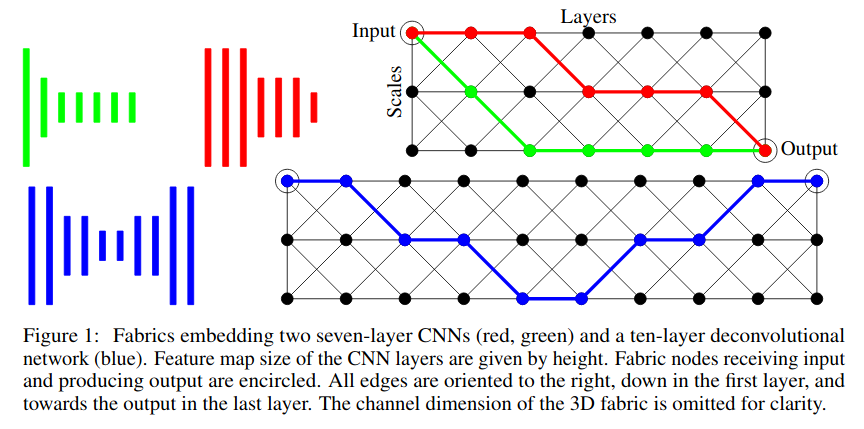
\includegraphics[width=0.7\textwidth]{images/conv_fabric.png}
	
	\begin{itemize}
	\footnotesize
		\item One path from the input to the output of the lattice determines the network structure.
		\item Paths (architectures) that overlap also share the parameters.
	\end{itemize}
	
}
%----------------------------------------------------------------------

%-----------------------------------------------------------------------
\myframetop{Weight sharing and one-shot models}{

\myit{
	\item All possible architectures are subgraphs of a large supergraph (the \alert{one-shot model})
	\item This one-shot model is \alert{trained as a standard neural network} with mini-batches and stochastic optimizers.
	\visible<2->{\item At each mini-batch iteration \alert{weights are shared} between different architectures with common edges/nodes in the supergraph}
	}
	
	\centering
	\visible<1->{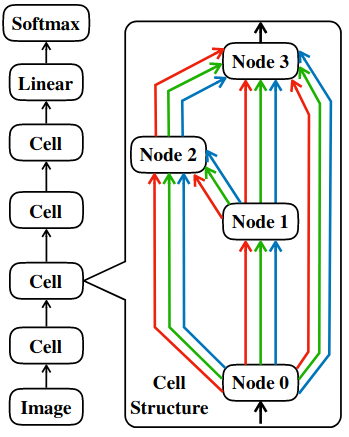
\includegraphics[width=0.2\textwidth]{images/one_shot_model_1.png}\quad\quad}
	\visible<2->{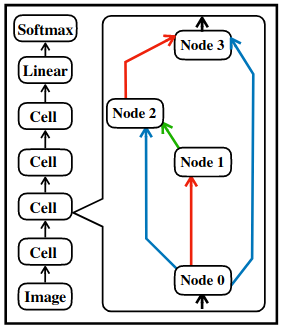
\includegraphics[width=0.2\textwidth]{images/one_shot_model_2.png}\quad\quad}
	\visible<3->{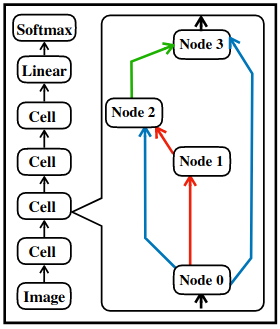
\includegraphics[width=0.2\textwidth]{images/one_shot_model_3.png}}

}
%----------------------------------------------------------------------

%-----------------------------------------------------------------------
%\myframetop{Basic Principle}{
%	\centering
%	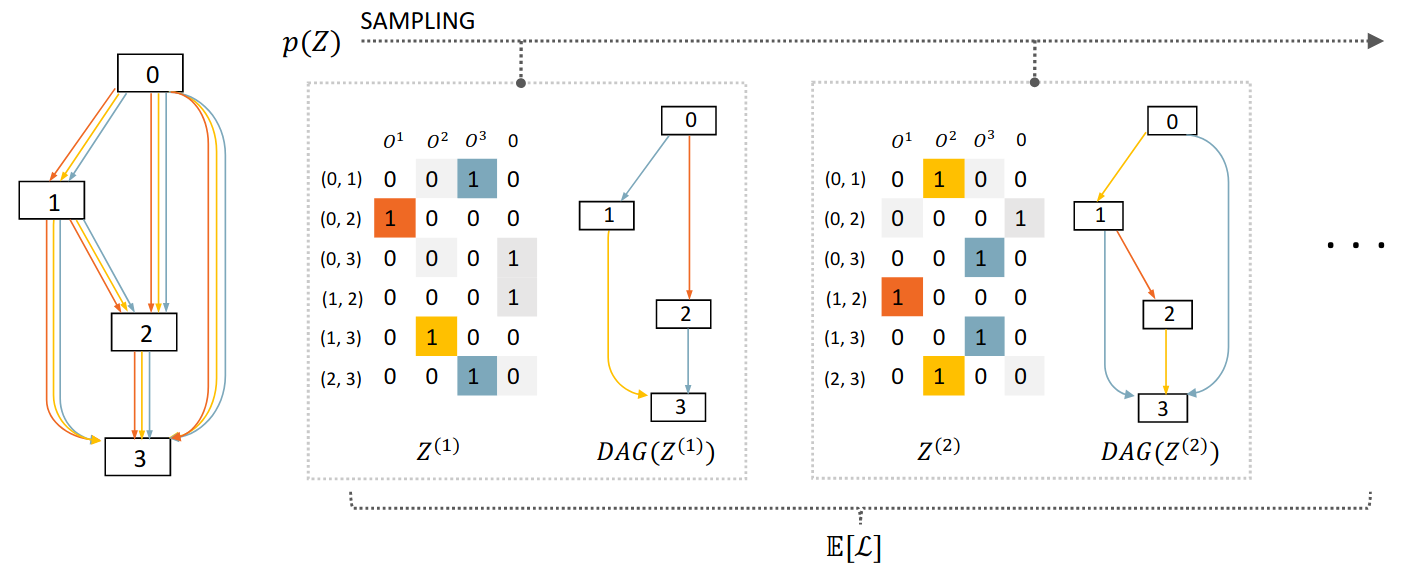
\includegraphics[width=0.7\textwidth]{images/snas_oneshot.png}
%	
%	\only<1>{
%	\begin{itemize}
%	\footnotesize
%		\item The \textbf{one-shot model} is a multi-graph containing all possible DAGs
%		\myit{
%		\footnotesize
%			\item[-] Every DAG represents a single architecture $Z^{(\cdot)}$ in the search space $\mathcal{A}$.
%			\item[-] Nodes represent aggregating operations (e.g. summation, concatenation) for incoming tensors.
%			\item[-] Edges represent operations $O^i$ (in the figure: one color per operation)
%			}
%		\item The row labels in the matrix above represent a pair of nodes $(j,k)$ in the graph and the column labels the operations $O^i$. A value of $1$ means that that operaration is active in the edge connecting node $j$ to $k$.
%	\end{itemize}
%	}
%	
%	\only<2>{
%	\begin{itemize}
%	\footnotesize
%		\item The most important principle in one-shot models is \textbf{weight-sharing} between graphs.
%		\myit{
%		\footnotesize
%			\item[-] The one-shot model is trained as a normal neural network, i.e. with mini-batch training. The question is how to distinguish single architectures in the one-shot model during this training?
%			\item[-] One way is that for each sampled mini-batch also sample stochastically an architecture (DAG) and update only the parameters of that architecture.
%			\item[-] For all subsequent iterations in case a new sampled architecture has common edges (i.e. some entries in the matrices are the same) in the DAG, the weights are shared.
%			}
%	\end{itemize}
%	}
%}
%----------------------------------------------------------------------

%----------------------------------------------------------------------

\myframetop{Training the one-shot model -- ScheduledDropPath \litw{\href{http://proceedings.mlr.press/v80/bender18a/bender18a.pdf}{Bender et al., 2018}}}{
	\centering
	
	\begin{itemize}
	%\footnotesize
		\item One way to train the one-shot model is as a normal neural network and use \alert{ScheduledDropPath}
		\myit{
			\item[-] Analogous to Dropout \lit{\href{http://jmlr.org/papers/v15/srivastava14a.html}{Srivastava et al., 2014}} in standard neural networks.
			\item[-] At each mini-batch iteration \alert{zero out every operation} connecting 2 nodes with probability $p$.
			\item[-] ScheduledDropPath starts with $p=0$ and increases that linearly throughout training until a maximum $p_{max}$ in the end.
			}
	\end{itemize}
	
	\centering
	\visible<1->{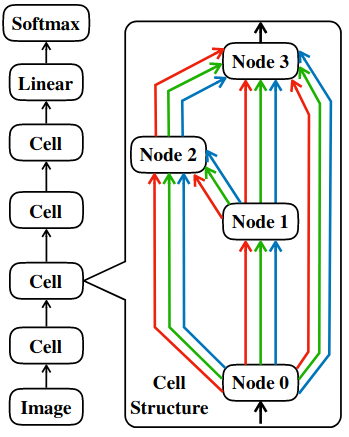
\includegraphics[width=0.2\textwidth]{images/one_shot_model_1.png}\quad\quad}
	\visible<1->{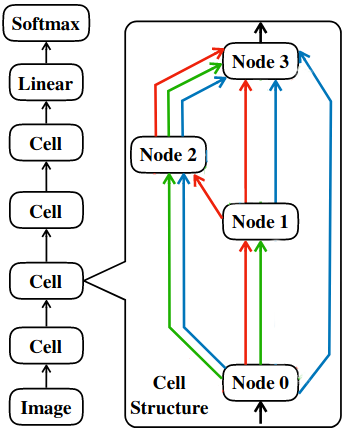
\includegraphics[width=0.2\textwidth]{images/drop_path_1.png}\quad\quad}
	\visible<2->{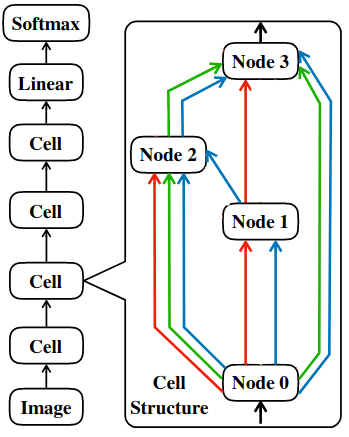
\includegraphics[width=0.2\textwidth]{images/drop_path_2.png}}
	
}
%----------------------------------------------------------------------

%----------------------------------------------------------------------

%\myframetop{Impact of DropPath \litw{\href{http://proceedings.mlr.press/v80/bender18a/bender18a.pdf}{Bender et al., 2018}}}{
%	\centering
%	
%	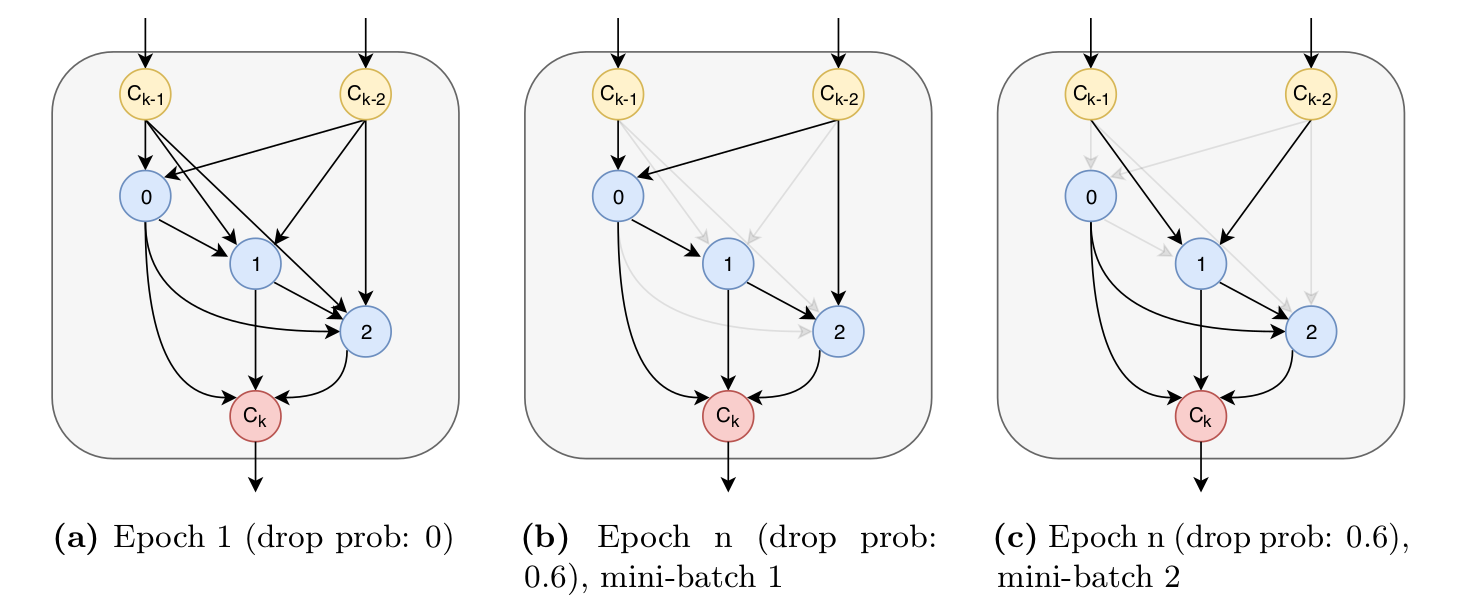
\includegraphics[width=0.8\textwidth]{images/droppath.png}
%	
%    \begin{itemize}
%		\item DropPath zeros out one a subset of the operations at each mini-batch training iteration with probability $p$.
%		\item ScheduledDropPath starts with $p=0$ and increases that linearly throughout training until a maximum $p_{max}$ in the end.
%	\end{itemize}
%}
%---------------------------------------------------------------


%----------------------------------------------------------------------

\myframetop{Training the one-shot model -- Sampling}{
	\centering
	
    \begin{itemize}
		\item At each mini-batch iteration during the training of the one-shot model sample one architecture $Z$ from the search space $\mathcal{A}$.
		\visible<2->{
		\myit{
			\item[-] \textbf{Random Search with Weight Sharing} \lit{\href{https://arxiv.org/pdf/1902.07638.pdf}{Li and Talwalkar, 2020}} $\longrightarrow$ sample from uniform distribution
			\item[-] \textbf{ENAS} \lit{\href{https://arxiv.org/pdf/1802.03268.pdf}{Pham et al., 2018}} $\longrightarrow$ sample from the learned policy of a RNN controller
		}
		}
		\item \alert{Update the parameters of the one-shot model} corresponding to only that architecture.
	\end{itemize}
	
	\only<1->{
	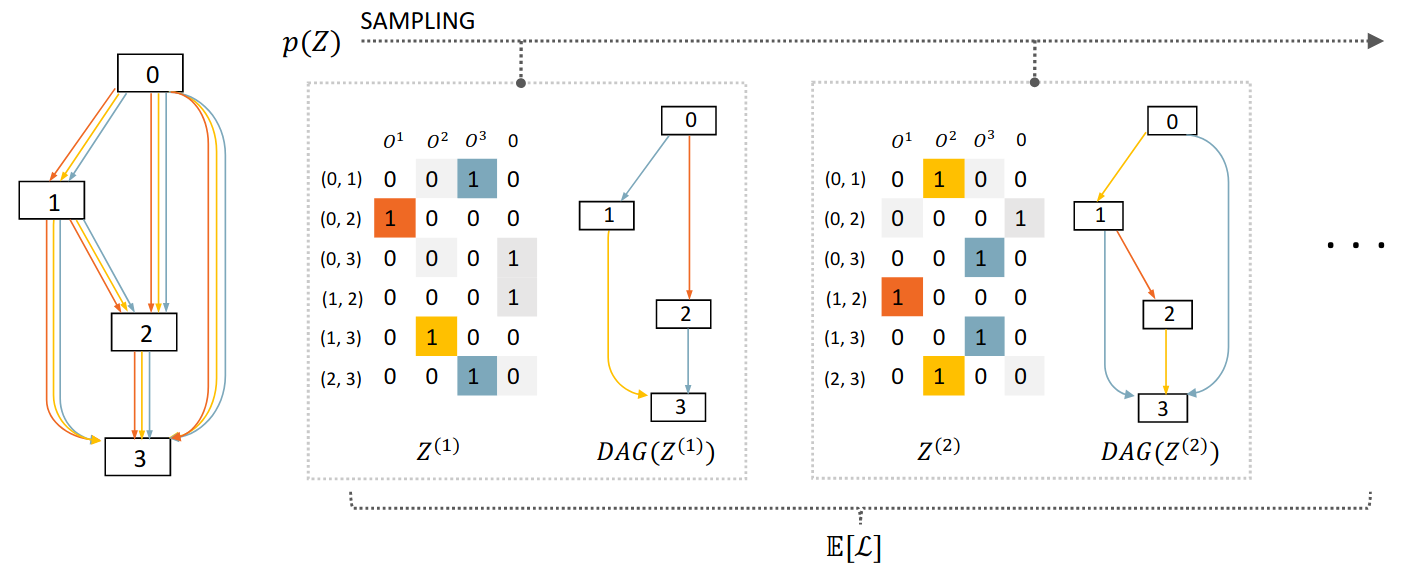
\includegraphics[width=.75\textwidth]{images/snas_oneshot.png}
	}
}
%---------------------------------------------------------------


%----------------------------------------------------------------------

%\myframetop{Random Search with Weight Sharing \litw{\href{https://arxiv.org/pdf/1902.07638.pdf}{Li and Talwalkar, 2020}}}{
%	\centering
	
%    \begin{itemize}
%		\item Random Search with Weight Sharing \textbf{utilizes the one-shot model to speed up vanilla random search} as follows:
%		\myit{
%			\only<1>{
%			\item[-] At each mini-batch iteration during the training of the one-shot model \alert{sample uniformly at random} one architecture $Z$ from the search space $\mathcal{A}$.
%			\item[-] \alert{Update the parameters of the one-shot model} corresponding to only that architecture.
%			\item[-] After training the one-shot model finishes, sample uniformly at random $M$ architectures and rank them based on the error on a single mini-batch from the validation set \alert{using the one-shot model parameters} (retraining from scratch is computationaly expensive).
%			\item[-] Select the top $K$, where $K < M$, and evaluate those on the full validation set, again using the one-shot parameters.
%			\item[-] Return the top performing architecture to \alert{retrain from scratch}.
%			}
%			\only<2>{
%			\item[-] Works \alert{comparably to state-of-the-art NAS methods} on many benchmarks.
%			}
%		}
%	\end{itemize}
%	
%	\only<2>{
%	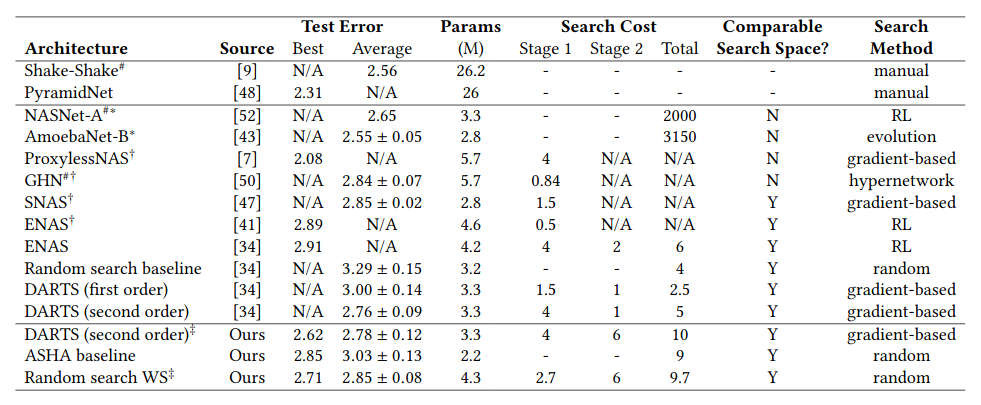
\includegraphics[width=.75\textwidth]{images/rs_ws.png}
%	}
%}
%---------------------------------------------------------------

\myframetop{How to utilize the trained one-shot model?}{
	\centering
	
    \begin{itemize}
		\item After training the one-shot model we have to \alert{select the best individual architecture} from that.
		\item There are multiple ways one can approach this. Some of these are:
		\myit{
			\item[$1$] Sample uniformly at random $M$ architectures and rank them based on the the validation error \alert{using the one-shot model parameters} (retraining from scratch is computationaly expensive).
			%\item[-] Select the top $K$, where $K < M$, and evaluate those on the full validation set, again using the one-shot parameters.
			\item[$1b$] (Optional) Select top $K$ ($K<M$) and retrain them from scratch for a couple of epochs.
			\item[$2$] Return the top performing architecture to \alert{retrain from scratch} for longer.
		}
	\end{itemize}
	
	\only<2>{
    	\begin{minipage}{0.4\textwidth}
        	\begin{itemize}
				\footnotesize
				\item \textbf{Pitfall:} the correlation between architectures evaluated with the one-shot weights and retrained from scratch (stand-alone models) should be high.
				\item If not, \textbf{selecting the best architecture based on the one-shot weights} is sub-optimal.
			\end{itemize}
	    \end{minipage}
	    \hspace{1cm}
    	\begin{minipage}{0.5\textwidth}
	        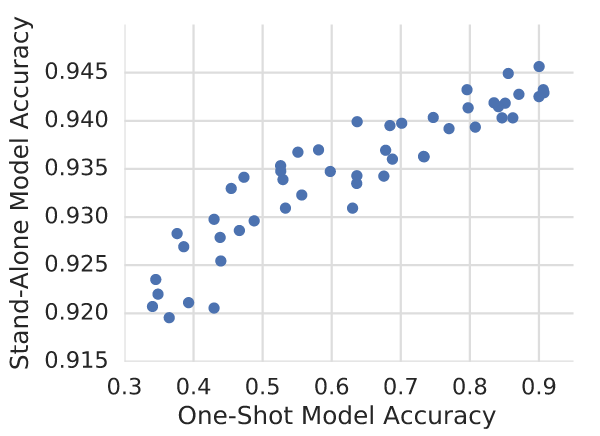
\includegraphics[width=.75\textwidth]{images/bender_correlation_1.png}    	
    	\end{minipage}
	}
}
%---------------------------------------------------------------

%----------------------------------------------------------------------
\myframe{Questions to Answer for Yourself / Discuss with Friends}{

	\myit{
		\item Repetition:\\ \alert{How are the weights shared in the one-shot model?}
\bigskip
		\item Repetition:\\ \alert{What is the difference between Random Search with Weight Sharing and ENAS?}
\medskip
		\item Repetition:\\ \alert{What are some pros and cons of using the one-shot model for NAS?}
	}	 
}
%-----------------------------------------------------------------------

